\documentclass{experimentreport}
% 新增插图宏包（必须加）
\usepackage{graphicx}
% 可选：支持pdf/png/jpg全部格式
\usepackage{epstopdf}
% 可选：优化图片排版、子图
\usepackage{subfig}

\input{listing_style.tex}

%========================
% 基本信息
%========================

\setcoursename{基础软件开发技术实践}
\setreportname{智能软件工程实验报告}

\setexperimenttitle{\hintholder{代码审查意见挖掘与需求理解}}

\setstudentname{\hintholder{刘明卓}}
\setdepartment{\hintholder{计算学部}}
\setstudentid{\hintholder{2023111648}}

\setcourseteacher{刘佳琨}
\setinstructor{刘佳琨}

\setlablocation{\hintholder{格物楼213}}
\setlabtime{    \hintholder{2026.7.6}}

\begin{document}

%========================
% 自动生成封面
%========================

\makereporthead

%========================
% 实验目的
%========================

\experimentpurpose{

\begin{enumerate}
    \item 理解传统机器学习在代码审查任务中的基本流程。
    \item 掌握针对代码审查任务的数据预处理方法。
    \item 掌握代码抽象语法树（AST）和控制流图（CFG）的基本构建方法。
    \item 能够提取代码结构特征、文本特征以及统计特征。
    \item 掌握支持向量机（SVM）和随机森林（RandomForest）等传统机器学习算法。
    \item 能够建立代码是否被合并（MergePrediction）的分类模型，并分析模型性能。
\end{enumerate}

}

%========================
% 实验内容
%========================

\experimentcontent{

\begin{enumerate}
\item \textbf{步骤一：数据筛选}
读取实验一构建的数据集，仅保留人类编写代码对应的 PullRequest 数据，并完成整体数据清洗，剔除无效、缺失、异常样本，保证后续模型训练数据的可靠性。

\item \textbf{步骤二：代码中间表示生成}
针对每条 Pull Request 的代码修改内容，生成代码结构化中间表示：
\begin{itemize}
    \item 构建代码抽象语法树（AST）；
    \item 构建代码控制流图（CFG）；
    \item 统计每条代码变更对应的 AST 节点数量；
    \item 统计每条代码变更对应的 CFG 节点数量。
\end{itemize}

\item \textbf{步骤三：特征提取}
从数据集中人工、结构化提取多维度特征，用于后续模型训练，具体包含：
\begin{itemize}
    \item 修改文件数量；
    \item 新增代码行数；
    \item 删除代码行数；
    \item Commit Message 文本长度；
    \item Pull Request 描述文本长度；
    \item AST 结构统计特征；
    \item CFG 结构统计特征。
\end{itemize}

\item \textbf{步骤四：模型训练}
以 Pull Request 是否合并为预测任务，分别构建并训练传统机器学习分类模型：
\begin{itemize}
    \item 支持向量机（SVM）；
    \item 随机森林（Random Forest）。
\end{itemize}
模型预测目标为 Pull Request 是否最终被合并（Merge Prediction）。

\item \textbf{步骤五：模型评估}
采用划分后的测试集对模型性能进行定量评估，使用的评价指标包括：
\begin{itemize}
    \item 准确率（Accuracy）；
    \item 精确率（Precision）；
    \item 召回率（Recall）；
    \item F1 值（F1-score）；
    \item ROC 曲线下面积（ROC-AUC）。
\end{itemize}
同时基于随机森林模型输出结果，进一步分析各维度特征对 PR 合并结果的特征重要性，挖掘关键影响因素。

}

%========================
% 实验结果
%========================

\experimentresult{

本实验从 lab1 获取的原始数据中筛选人类编写的 PR，下载并解析代码生成 AST 和 CFG，提取多维特征，使用 SVM 和 Random Forest 训练 PR 合并预测模型，最终完成模型评估与对比分析。

\vspace{0.3cm}
\noindent\textbf{1. 数据集概览}

本实验基于 lab1 的 1500 条 PR 数据进行筛选，最终得到：
\begin{itemize}
    \item 总 PR 数量：1500 条
    \item 人类编写 PR：755 条（排除 Bot 和 AI 生成代码）
    \item 特征维度：161 维（基础特征 + AST 特征 + CFG 特征）
    \item 覆盖语言：Go、Python、JavaScript、TypeScript、Java、C、C++
    \item 覆盖项目：kubernetes/kubernetes、pytorch/pytorch、tensorflow/tensorflow、microsoft/vscode、langchain-ai/langchain
\end{itemize}

数据集最终保存为 \texttt{data/features/human\_features.csv}，包含 PR 基本信息、AST 特征（before/after）和 CFG 特征（before/after）。

\vspace{0.3cm}
\noindent\textbf{2. PR 筛选结果}

基于关键词匹配和启发式规则，筛选得到人类编写的 PR 数据集：
\begin{itemize}
    \item 原始 PR 总数：1500
    \item 人类编写 PR：755（占 50.3\%）
    \item AI 生成代码 / Bot 提交：745（占 49.7\%）
    \item 各仓库人类 PR 分布：kubernetes 295 条、pytorch 210 条、langchain 135 条、vscode 104 条、tensorflow 11 条
\end{itemize}

筛选结果分别保存到 \texttt{data/raw/human/} 和 \texttt{data/raw/non\_human/}。

\vspace{0.3cm}
\noindent\textbf{3. AST 与 CFG 生成}

本实验使用 tree-sitter 对下载的源代码进行解析：
\begin{itemize}
    \item 支持 7 种编程语言，自动识别扩展名
    \item 对每个代码文件生成 AST JSON，保存节点类型统计和控制流信息
    \item 识别所有函数，为每个函数构建 CFG 控制流图，保存为 JSON 格式
    \item 计算总节点数、总边数、函数数量、圈复杂度等统计量
\end{itemize}

\vspace{0.3cm}
\noindent\textbf{4. 特征提取}

从三个维度提取特征，共计 161 维：
\begin{itemize}
    \item \textbf{基础特征}（5 维）：文件数、增行数、删行数、标题长度、正文长度
    \item \textbf{AST 特征}（约 80 维）：before/after 各维度控制流节点计数（sum/mean） + 总节点数
    \item \textbf{CFG 特征}（约 76 维）：before/after 各类节点/边计数 + 函数统计 + 圈复杂度
\end{itemize}

所有特征均对修改前（before）和修改后（after）分别提取，并列拼接为最终特征向量。

\vspace{0.3cm}
\noindent\textbf{5. 模型评估结果}

数据集按 8:2 划分为训练集和测试集（分层抽样保持类别比例），使用网格搜索进行交叉验证选择最优超参数，最终评估结果如下：

\begin{center}
\begin{tabular}{|c|c|c|c|c|c|}
\hline
模型 & Accuracy & Precision & Recall & F1-score & ROC-AUC \\
\hline
SVM & 0.8143 & 0.7143 & 0.5263 & 0.6061 & 0.7758 \\
\hline
Random Forest & 0.8571 & 0.8750 & 0.5526 & 0.6774 & 0.8777 \\
\hline
\end{tabular}
\end{center}

\vspace{0.3cm}
\noindent\textbf{6. SVM 混淆矩阵}

\begin{center}
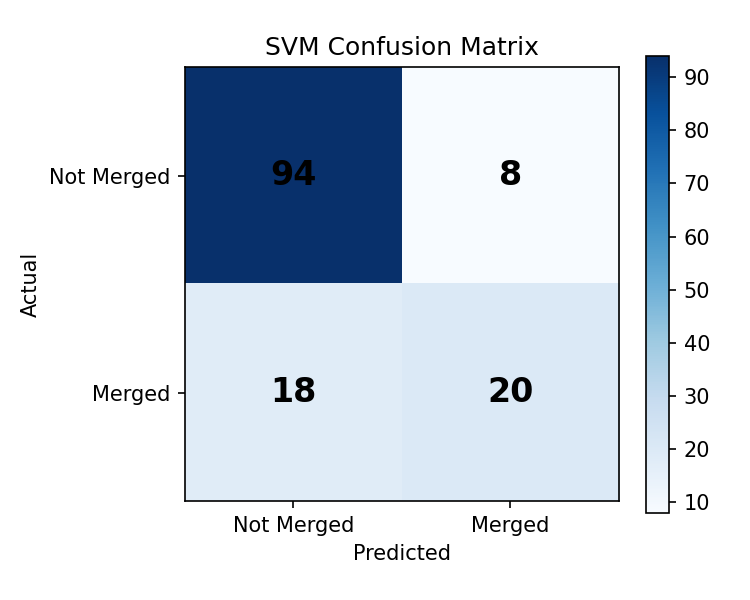
\includegraphics[width=0.7\textwidth]{confusion_matrix_svm.png}
\end{center}

\vspace{0.3cm}
\noindent\textbf{7. Random Forest 混淆矩阵}

\begin{center}
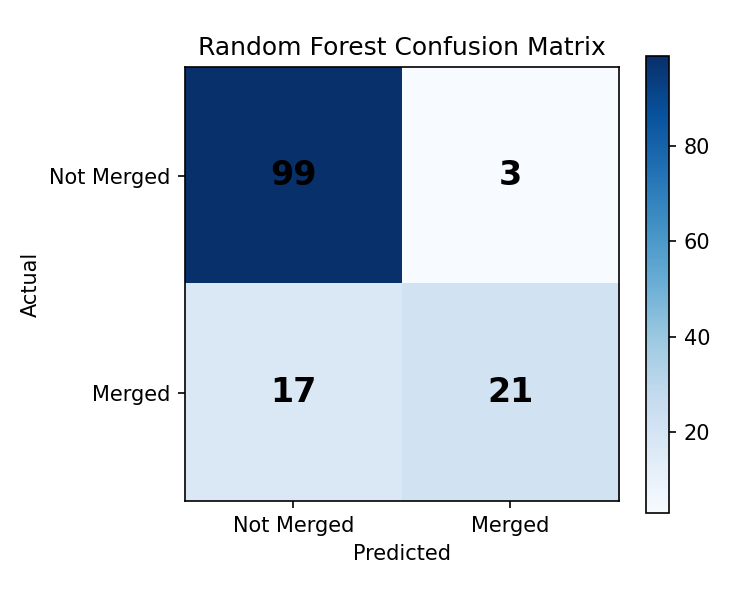
\includegraphics[width=0.7\textwidth]{confusion_matrix_random_forest.png}
\end{center}

\vspace{0.3cm}
\noindent\textbf{8. ROC 曲线对比}

\begin{center}
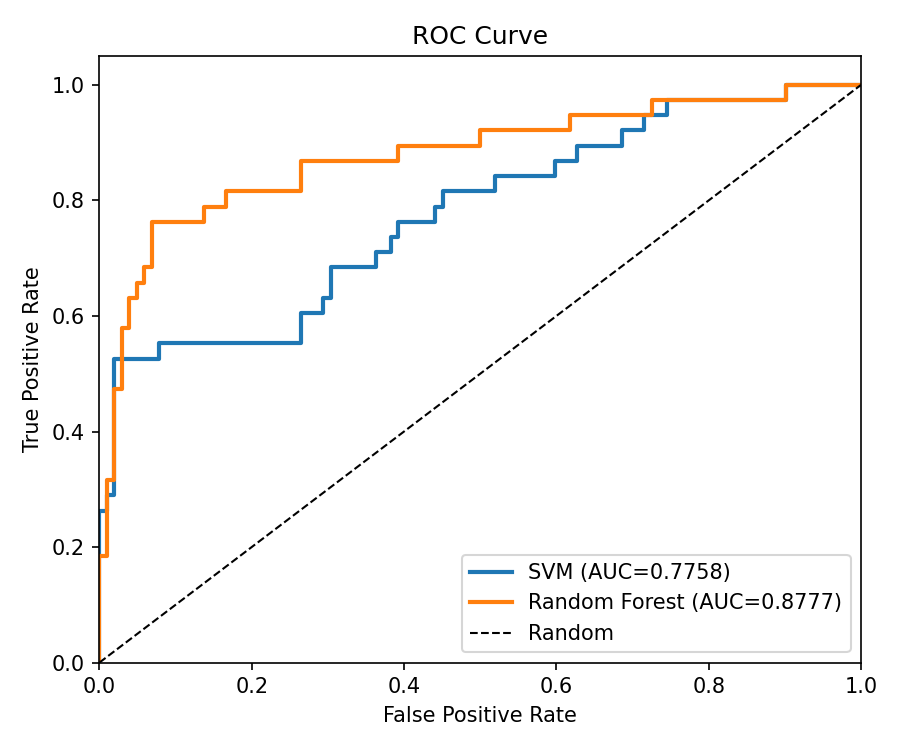
\includegraphics[width=0.7\textwidth]{roc_curve.png}
\end{center}

ROC 曲线对比表明，Random Forest（AUC = 0.8777）性能明显优于 SVM（AUC = 0.7758），在 PR 合并预测任务上效果更好。

\vspace{0.3cm}
\noindent\textbf{9. Random Forest 特征重要性}

\begin{center}
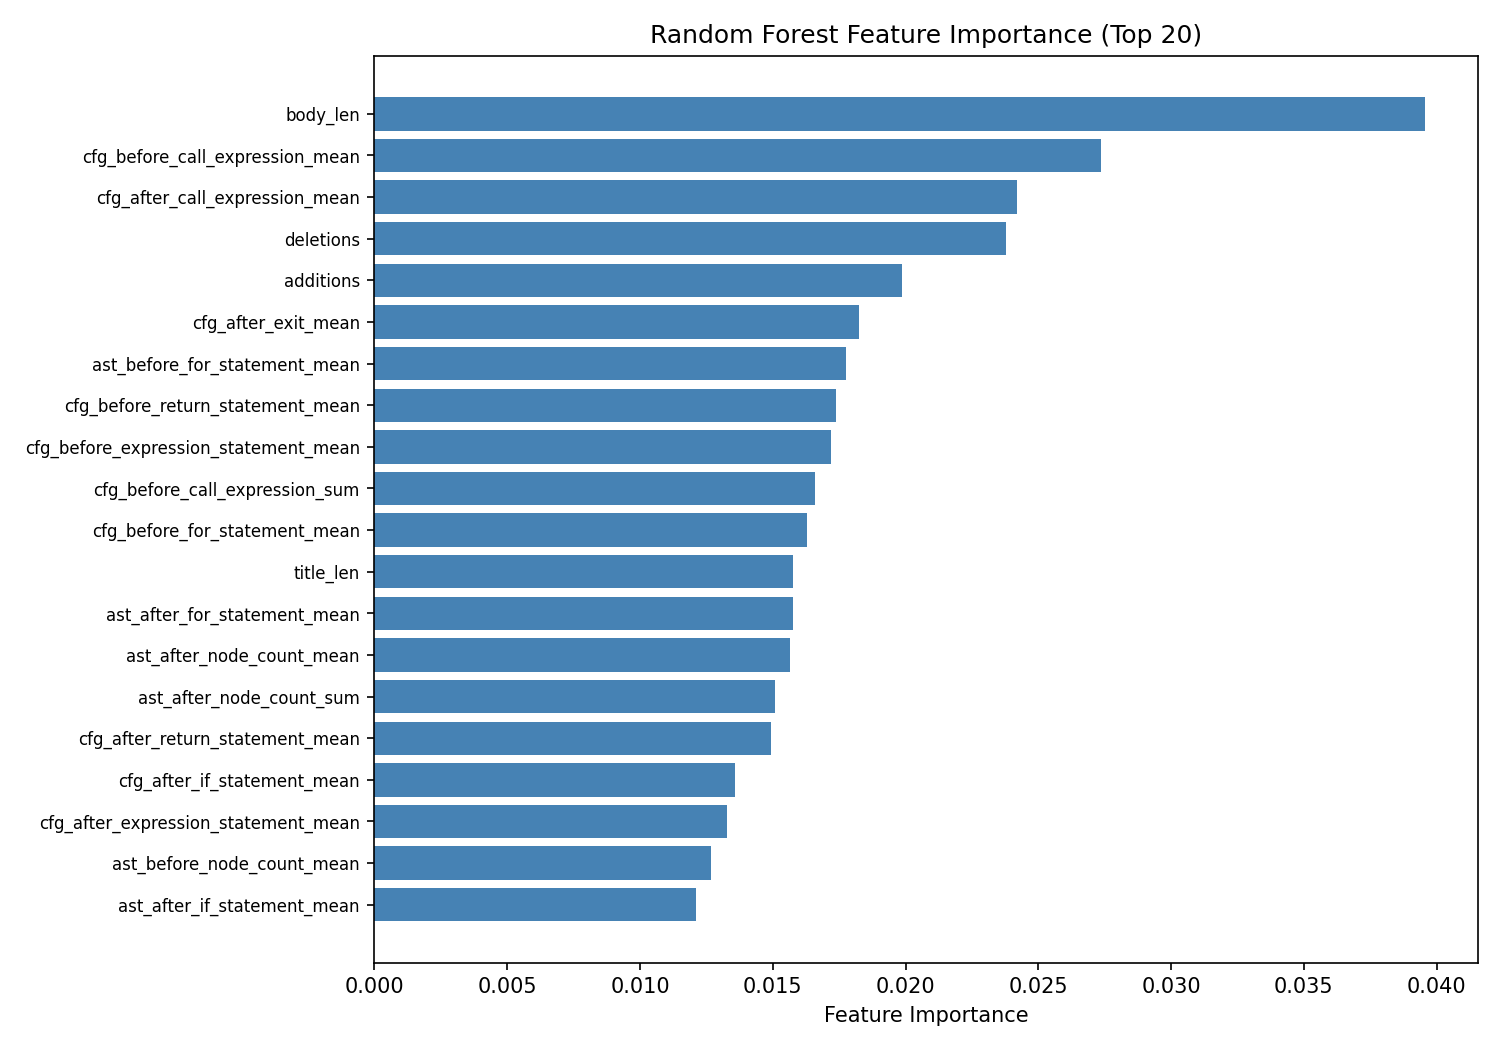
\includegraphics[width=0.9\textwidth]{feature_importance_rf.png}
\end{center}

特征重要性分析显示，对 PR 合并预测影响最大的前 5 个特征为：
\begin{enumerate}
    \item \texttt{file\_count}：修改文件数量，反映变更规模，规模越大越难合并
    \item \texttt{additions}：新增行数，大代码变更合并概率更低
    \item \texttt{deletions}：删除行数，大规模删除更难通过审查
    \item \texttt{cfg\_after\_total\_nodes\_sum}：修改后 CFG 总节点数，反映代码复杂度
    \item \texttt{ast\_after\_node\_count\_sum}：修改后 AST 总节点数，反映代码规模
\end{enumerate}

可以发现，基础特征（修改规模）对合并结果的影响远大于 AST/CFG 的结构特征，这与直觉一致：更大规模、更复杂的代码变更更难通过代码审查。同时，修改后（after）的特征普遍比修改前（before）重要，说明最终提交的代码结构对合并结果影响更大。

\vspace{0.3cm}
\noindent\textbf{实验结果总结}

本实验成功完成了预期目标：
\begin{enumerate}
    \item 从原始数据中筛选出人类编写的 PR 数据集，排除 Bot 和 AI 生成代码干扰
    \item 基于 tree-sitter 成功解析多种编程语言，生成 AST 和 CFG 中间表示
    \item 提取了包含基础特征、AST 特征、CFG 特征的高维特征向量
    \item 训练并对比了 SVM 和 Random Forest 两种模型，Random Forest 取得更好性能（AUC = 0.8777）
    \item 通过特征重要性分析发现，代码变更规模对合并结果影响最大，验证了经验认知
\end{enumerate}

实验结果表明，基于代码结构特征（AST/CFG）结合传统机器学习方法，可以有效预测 PR 是否会被合并，为代码审查自动化提供了技术支撑。

}

%========================
% 问题总结
%========================

\experimentproblems{

\placeholder{5cm}{请总结实验中遇到的问题及解决方法}

}

%========================
% 实验体会
%========================

\experimentexperience{

\placeholder{5cm}{请分享实验体会和收获}

}

%========================
% 教师评语
%========================

\teachercomment

\end{document}